\documentclass{article}\usepackage[]{graphicx}\usepackage[]{color}
%% maxwidth is the original width if it is less than linewidth
%% otherwise use linewidth (to make sure the graphics do not exceed the margin)
\makeatletter
\def\maxwidth{ %
  \ifdim\Gin@nat@width>\linewidth
    \linewidth
  \else
    \Gin@nat@width
  \fi
}
\makeatother

\definecolor{fgcolor}{rgb}{0.345, 0.345, 0.345}
\newcommand{\hlnum}[1]{\textcolor[rgb]{0.686,0.059,0.569}{#1}}%
\newcommand{\hlstr}[1]{\textcolor[rgb]{0.192,0.494,0.8}{#1}}%
\newcommand{\hlcom}[1]{\textcolor[rgb]{0.678,0.584,0.686}{\textit{#1}}}%
\newcommand{\hlopt}[1]{\textcolor[rgb]{0,0,0}{#1}}%
\newcommand{\hlstd}[1]{\textcolor[rgb]{0.345,0.345,0.345}{#1}}%
\newcommand{\hlkwa}[1]{\textcolor[rgb]{0.161,0.373,0.58}{\textbf{#1}}}%
\newcommand{\hlkwb}[1]{\textcolor[rgb]{0.69,0.353,0.396}{#1}}%
\newcommand{\hlkwc}[1]{\textcolor[rgb]{0.333,0.667,0.333}{#1}}%
\newcommand{\hlkwd}[1]{\textcolor[rgb]{0.737,0.353,0.396}{\textbf{#1}}}%

\usepackage{framed}
\makeatletter
\newenvironment{kframe}{%
 \def\at@end@of@kframe{}%
 \ifinner\ifhmode%
  \def\at@end@of@kframe{\end{minipage}}%
  \begin{minipage}{\columnwidth}%
 \fi\fi%
 \def\FrameCommand##1{\hskip\@totalleftmargin \hskip-\fboxsep
 \colorbox{shadecolor}{##1}\hskip-\fboxsep
     % There is no \\@totalrightmargin, so:
     \hskip-\linewidth \hskip-\@totalleftmargin \hskip\columnwidth}%
 \MakeFramed {\advance\hsize-\width
   \@totalleftmargin\z@ \linewidth\hsize
   \@setminipage}}%
 {\par\unskip\endMakeFramed%
 \at@end@of@kframe}
\makeatother

\definecolor{shadecolor}{rgb}{.97, .97, .97}
\definecolor{messagecolor}{rgb}{0, 0, 0}
\definecolor{warningcolor}{rgb}{1, 0, 1}
\definecolor{errorcolor}{rgb}{1, 0, 0}
\newenvironment{knitrout}{}{} % an empty environment to be redefined in TeX

\usepackage{alltt}
\IfFileExists{upquote.sty}{\usepackage{upquote}}{}
\begin{document}

\begin{knitrout}
\definecolor{shadecolor}{rgb}{0.969, 0.969, 0.969}\color{fgcolor}\begin{kframe}
\begin{alltt}
\hlkwd{library}\hlstd{(ggplot2)}
\hlkwd{library}\hlstd{(ggmap)}
\end{alltt}


{\ttfamily\noindent\color{warningcolor}{\#\# Warning: package 'ggmap' was built under R version 3.2.5}}\begin{alltt}
\hlkwd{library}\hlstd{(raster)}
\end{alltt}


{\ttfamily\noindent\color{warningcolor}{\#\# Warning: package 'raster' was built under R version 3.2.5}}

{\ttfamily\noindent\itshape\color{messagecolor}{\#\# Loading required package: sp}}

{\ttfamily\noindent\color{warningcolor}{\#\# Warning: package 'sp' was built under R version 3.2.5}}\begin{alltt}
\hlkwd{library}\hlstd{(sp)}
\hlkwd{library}\hlstd{(rgdal)}
\end{alltt}


{\ttfamily\noindent\color{warningcolor}{\#\# Warning: package 'rgdal' was built under R version 3.2.5}}

{\ttfamily\noindent\itshape\color{messagecolor}{\#\# rgdal: version: 1.1-10, (SVN revision 622)\\\#\#\ \ Geospatial Data Abstraction Library extensions to R successfully loaded\\\#\#\ \ Loaded GDAL runtime: GDAL 2.0.1, released 2015/09/15\\\#\#\ \ Path to GDAL shared files: C:/Users/Timothee/Documents/R/win-library/3.2/rgdal/gdal\\\#\#\ \ GDAL does not use iconv for recoding strings.\\\#\#\ \ Loaded PROJ.4 runtime: Rel. 4.9.1, 04 March 2015, [PJ\_VERSION: 491]\\\#\#\ \ Path to PROJ.4 shared files: C:/Users/Timothee/Documents/R/win-library/3.2/rgdal/proj\\\#\#\ \ Linking to sp version: 1.2-3}}\begin{alltt}
\hlkwd{library}\hlstd{(RColorBrewer)}

\hlkwd{setwd}\hlstd{(}\hlkwc{dir} \hlstd{=} \hlstr{"D:/Documents/GitHub/PhDThesis-writing/FiguresGeneral/Map/"}\hlstd{)}

\hlstd{cpal} \hlkwb{<-} \hlkwd{brewer.pal}\hlstd{(}\hlkwc{n}\hlstd{=}\hlnum{6}\hlstd{,} \hlkwc{name}\hlstd{=}\hlstr{"Greys"}\hlstd{)}

\hlstd{CH_borders} \hlkwb{<-} \hlkwd{getData}\hlstd{(}\hlstr{"GADM"}\hlstd{,} \hlkwc{country}\hlstd{=}\hlstr{"CH"}\hlstd{,} \hlkwc{level}\hlstd{=}\hlnum{0} \hlstd{)}
\hlstd{AT_borders} \hlkwb{<-} \hlkwd{getData}\hlstd{(}\hlstr{"GADM"}\hlstd{,} \hlkwc{country}\hlstd{=}\hlstr{'AT'}\hlstd{,} \hlkwc{level}\hlstd{=}\hlnum{0}\hlstd{)}
\hlstd{LI_borders} \hlkwb{<-} \hlkwd{getData}\hlstd{(}\hlstr{"GADM"}\hlstd{,} \hlkwc{country}\hlstd{=}\hlstr{'LI'}\hlstd{,} \hlkwc{level}\hlstd{=}\hlnum{0}\hlstd{)}
\hlstd{IT_borders} \hlkwb{<-} \hlkwd{getData}\hlstd{(}\hlstr{"GADM"}\hlstd{,} \hlkwc{country}\hlstd{=}\hlstr{'IT'}\hlstd{,} \hlkwc{level}\hlstd{=}\hlnum{0}\hlstd{)}
\hlstd{DE_borders} \hlkwb{<-} \hlkwd{getData}\hlstd{(}\hlstr{"GADM"}\hlstd{,} \hlkwc{country}\hlstd{=}\hlstr{'DE'}\hlstd{,} \hlkwc{level}\hlstd{=}\hlnum{0}\hlstd{)}
\hlstd{FR_borders} \hlkwb{<-} \hlkwd{getData}\hlstd{(}\hlstr{"GADM"}\hlstd{,} \hlkwc{country}\hlstd{=}\hlstr{'FR'}\hlstd{,} \hlkwc{level}\hlstd{=}\hlnum{0}\hlstd{)}
\end{alltt}
\end{kframe}
\end{knitrout}


\begin{knitrout}
\definecolor{shadecolor}{rgb}{0.969, 0.969, 0.969}\color{fgcolor}\begin{kframe}


{\ttfamily\noindent\color{warningcolor}{\#\# Warning: package 'maps' was built under R version 3.2.5}}

{\ttfamily\noindent\color{warningcolor}{\#\# Warning: package 'GISTools' was built under R version 3.2.5}}

{\ttfamily\noindent\itshape\color{messagecolor}{\#\# Loading required package: maptools}}

{\ttfamily\noindent\color{warningcolor}{\#\# Warning: package 'maptools' was built under R version 3.2.5}}

{\ttfamily\noindent\itshape\color{messagecolor}{\#\# Checking rgeos availability: TRUE}}

{\ttfamily\noindent\itshape\color{messagecolor}{\#\# Loading required package: MASS}}

{\ttfamily\noindent\itshape\color{messagecolor}{\#\# \\\#\# Attaching package: 'MASS'}}

{\ttfamily\noindent\itshape\color{messagecolor}{\#\# The following objects are masked from 'package:raster':\\\#\# \\\#\#\ \ \ \  area, select}}

{\ttfamily\noindent\itshape\color{messagecolor}{\#\# Loading required package: rgeos}}

{\ttfamily\noindent\color{warningcolor}{\#\# Warning: package 'rgeos' was built under R version 3.2.5}}

{\ttfamily\noindent\itshape\color{messagecolor}{\#\# rgeos version: 0.3-19, (SVN revision 524)\\\#\#\ \ GEOS runtime version: 3.5.0-CAPI-1.9.0 r4084 \\\#\#\ \ Linking to sp version: 1.2-3 \\\#\#\ \ Polygon checking: TRUE}}\end{kframe}

{\centering 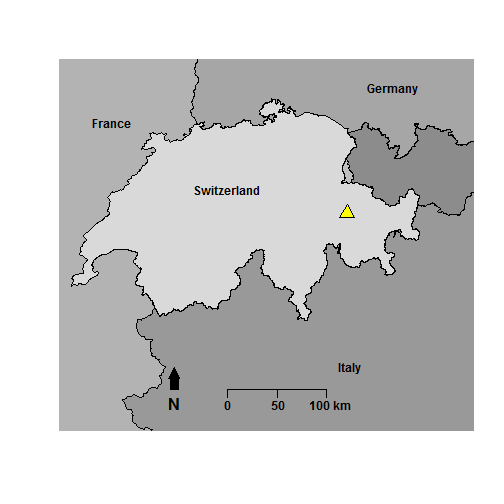
\includegraphics[width=1\textwidth]{figure/map-1} 

}



\end{knitrout}


\end{document}
